\documentclass[pdftex, a4paper]{scrartcl}
\usepackage[a4paper, total={6in, 11in}]{geometry}
\usepackage{ngerman}
\usepackage[utf8]{inputenc}
\usepackage[T1]{fontenc}
%x\usepackage{parskip}
\usepackage{array}
\usepackage {graphicx}
\usepackage{mathtools}

\begin{document}

\section{Organization}

\begin{itemize}
    \item Name: Bruno Macedo da Silva
    \item Student-ID: 676857
    \item Course: 506 Software Architektur 
    \item Semester: 5th
    \item Topic: ``Fast food delivery service - web and/or mobile application with backend and business functionality''
    \item Group A: 
        \begin{itemize}
            \item Tom Braum - ``Distributed, scalable software architecture for massively-multiplayer online (app or 
            client-based) games''
            \item Benjamin - ``Distributed, scalable software architecture for massively-multiplayer online (app or 
            client-based) games''
        \end{itemize}
\end{itemize}

\section{Preliminary Idea}

The main idea of this project is to develop a mobile application that contributes to the reduce of food waste 
in restaurants and bakeries. We want to offer a platform where these shops can log, register themselves and offer
products that were not consumed on the current day, but are still fresh and at the same time would not be sold on 
the next day. These products should cost much less as the normal price.

Users would have the option to log, register themselves and browse on the app to see what restaurant or bakeries
are offering remaining products. They would also see up to what time their purchase may be collected.

Similar application that were used as inspiration are as Inspiration were ``Too Good to Go'', ``ShareTheMeal'' 
and ``Food to Save''.

\begin{figure}[htb]
    \centering
    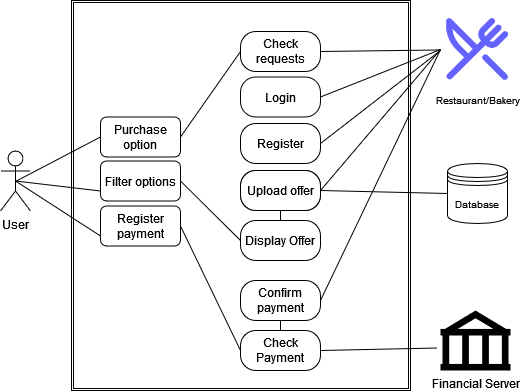
\includegraphics[width=0.50\textwidth]{/home/bruno/git/Soft.Arch/assets/preliminary_use_case.png}
    \caption{Preliminary description of the application}
    \label{fig:predes}
\end{figure}

\section{Architectural Drivers}

\begin{itemize}
    \item \textbf{Design Purpose}: general acceptance by potential clients and restaurants/bakeries, used
    time and money to develop a final project that attend an initial demand
    \item \textbf{Quality Attributes}: usability, availability, modifiability, security
    \item \textbf{Preliminary Functionality}: input of availability of restaurant/bakery, select restaurant/bakery, 
    register payment
    \item \textbf{Architectural Concerns}: programming language, connection with payment server, authentication
    \item \textbf{Constraints}: time, financial, platform (iOS, Android)
\end{itemize}

\end{document}
